\documentclass[swedish]{article}

\usepackage[a4paper,left=1in,right=1in,top=1.25in,bottom=1.25in]{geometry}
\usepackage[style=iso]{datetime2}
\usepackage{graphicx}
\usepackage{amssymb}

\author{Arvid Karlgren}
\title{Föreläsning 1\\
       \LARGE Gränsvärden: Definition och räkneregler}

\renewcommand{\contentsname}{Innehåll}
\setlength\parindent{0pt}

\begin{document}

\maketitle

\tableofcontents

\pagebreak

\section{Kursens mål}

Kursen kommer att hantera följande områden:

\begin{enumerate}
    \item Kontinuitet
    \item Gränsvärden
    \item Derivata
    \item Funktionsundersökning
    \item Primitiva funktioner
    \item Integraler
\end{enumerate}

\pagebreak

\section{Gränsvärden}

\subsection{Definition}

Gränsvärden handlar om hur en funktion ser ut (vilka värden den antar) när x närmar sig olika värden. Det finns två typer av gränsvärden.

\begin{itemize}
    \item{Nära (men ej i) en punkt $a\in x$.}
    \item{För obegränsat stora positiva eller negativa $x\in \mathbb{R}$.}
\end{itemize}

Gränsvärden betecknas med $\to$, till exempel $x \to a$ ("$x$ går mot $a$").

Figur 1 visar några fall där den exakta definitionen av gränsvärden spelar stor roll. 

\begin{figure}[h!]
    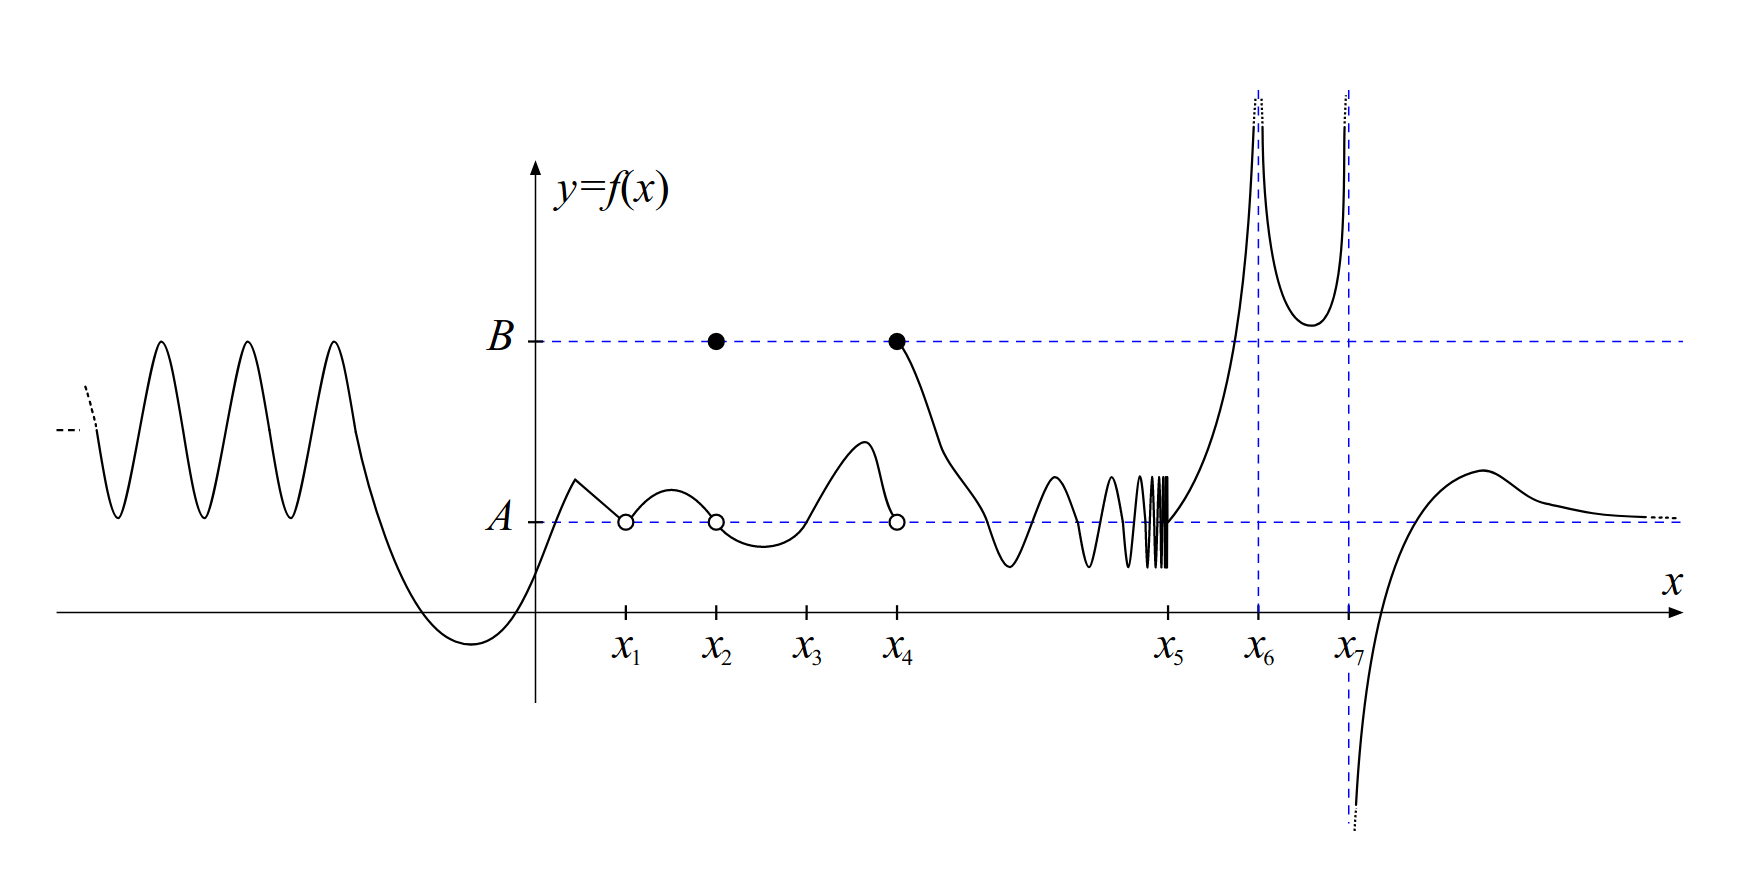
\includegraphics[width=\linewidth]{figur1.png}
    \label{fig:figur1}
    \caption{Olika fall för gränsvärden.}
\end{figure}

Utifrån figur 1 vill vi, utifrån definitionen för gränsvärden, kunna säga följande:

\begin{itemize}
    \item{$f(x) \to A$ då $x \to x_1$, ($x_1 \notin D_f$), skrivs $\lim\limits_{x \to x_1} f(x) = A$}
    \item{$f(x) \to A$ då $x \to x_2$, ($x_2 \in D_f$, $f(x_2) = B$).}
    \item{$f(x) \to A$ då $x \to x_3$, ($x_3 \in D_f$, $f(x_3) = A$).}
    \item{$f(x)$ saknar gränsvärden då $x \to x_4$ eller $x \to x_5$, skrivs $\lim\limits_{x \to x_4} f(x) \; \nexists$}
        \begin{itemize}
            \item{Däremot:\\

                $\lim\limits_{x \to x_4^-} = A \quad$ (Vänstergränsvärde, från vänster)\\

                $\lim\limits_{x \to x_4^+} = B \quad$ (Högergränsvärde, från höger)}
        \end{itemize}
    \item{$f(x) \to \infty$ då $x \to x_6$}
    \item{$f(x)$ saknar gränsvärde då $x \to x_7$}
    \item{$f(x) \to A$ då $x \to \infty$}
    \item{$f(x)$ saknar gränsvärde då $x \to -\infty$}
\end{itemize}

\bigbreak

{\Large\underline{$x \to a$}}

\smallbreak

\textbf{Definition:}

\smallskip

Gränsvärdet för $x \to a$ blir $A$, dvs. $\lim\limits_{x \to a} = A$ om det till varje $\epsilon < 0$ finns ett $\delta < 0$ sådant att $|f(x) - A| < \epsilon$ om $x \in D_f$ och $0 < |x - a| < \delta$ (se figur 2 nedan). 

\begin{figure}[h!]
    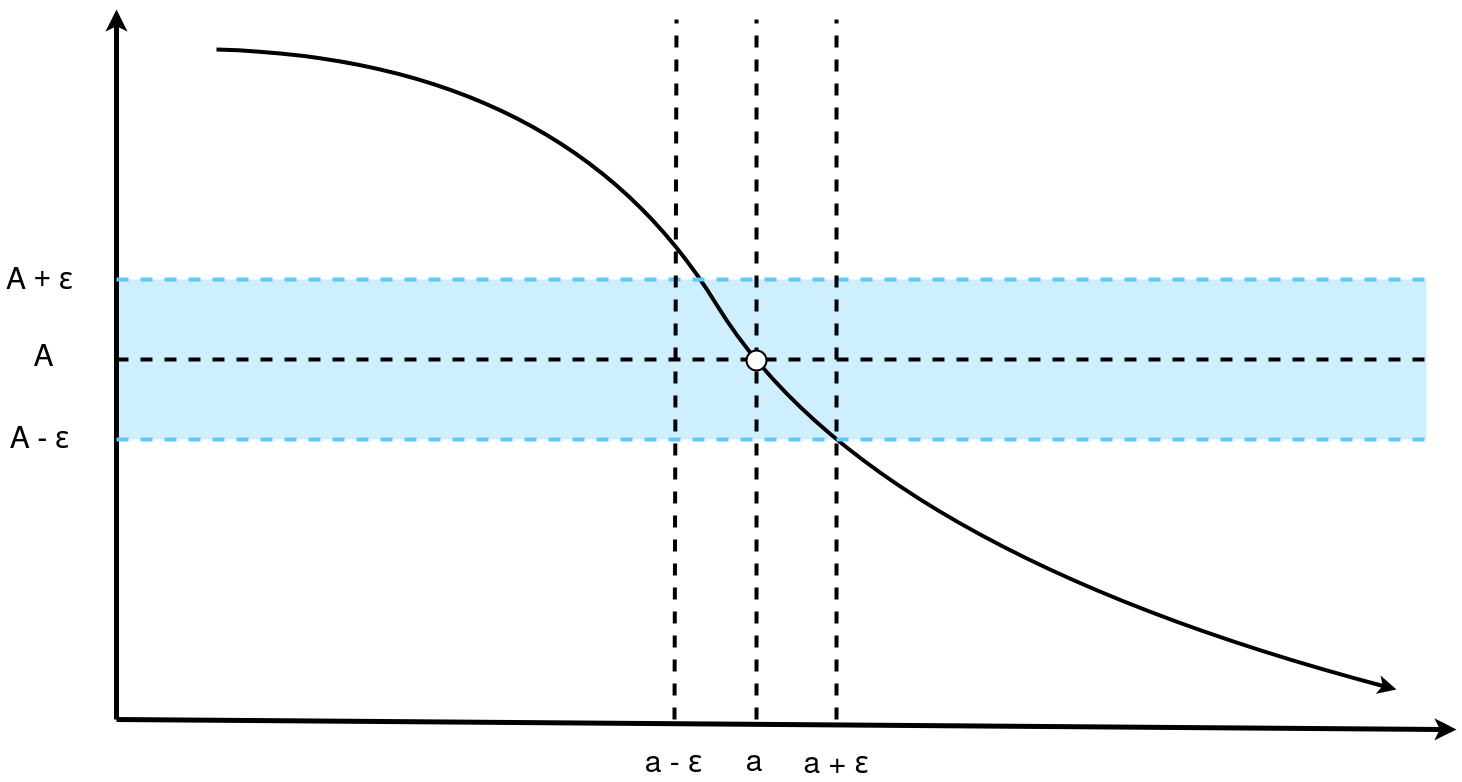
\includegraphics[width=\linewidth]{figur2.png}
    \label{fig:figure2}
    \caption{Definition av $x \to a$.}
\end{figure}

{\Large\underline{$x \to \infty$}}

\smallbreak

\textbf{Definition:}

Gränsvärdet för $x \to \infty$ blir $A$ om det till varje $\epsilon < 0$ finns ett $\omega$ sådant att $|f(x) - A| < \epsilon$ om $x \in D_f$ och $x > \omega$. \textbf{OBS!} krav finns på $D_f$, se boken. 

\subsubsection{Exempel}

\textbf{Visa att $\sqrt{x} \to \sqrt{a}$ då $x \to a$ och $a > 0$.}

Låt $\epsilon > 0$. Vi ska hitta passande $\delta$.

\[|\sqrt{x} - \sqrt{a}| = \left|\frac{x-a}{\sqrt{x}+\sqrt{a}}\right| \leq \left|\frac{x-a}{\sqrt{a}}\right|\]

\subsection{Räkneregler}

\end{document}
